\documentclass{beamer}

\usepackage{subfigure}
\usepackage{caption}
\usepackage{multirow}
\usepackage{array}
\usepackage[T1]{fontenc}

% using: https://github.com/matze/mtheme
\usetheme{metropolis}

\title{Improving the simulation of variable renewable energy in the MEDEAS integrated assessment model}
\date{September 4, 2023}

\author{François Straet}
\institute{University of Liège - School of Engineering and Computer Science}

\newcommand{\mysection}[1]{\section{\thesection. #1}}

% 150-160 words per minute

\begin{document}

    \maketitle

    \begin{frame}{Outline}
        \tableofcontents        
    \end{frame}

    \mysection{Models}
    \begin{frame}{Dispa-SET}
        \begin{itemize}
            \item Unit commitment model
            \item Formulated in linear programming
            \item Models the european grid
            \item Focus on renewable energy sources
            \item Open-source
        \end{itemize}

    \end{frame}

    \begin{frame}{Dispa-SET}
        \begin{figure}
            \centering
            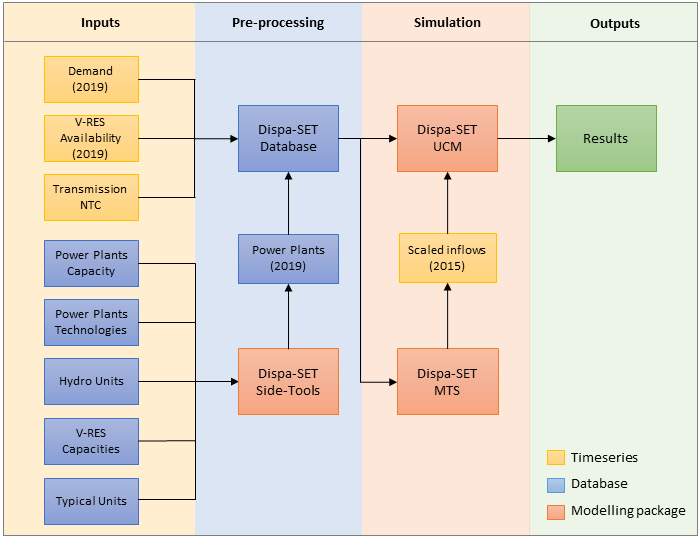
\includegraphics[width=0.7\textwidth]{../resources/images/dispaset-architecture.png}
            \caption{Block diagram of the architecture of the Dispa-SET model}
        \end{figure}
    \end{frame}

    \begin{frame}{MEDEAS}
        Modelling the Energy Development under Environmental And Socioeconomic constraints (MEDEAS)
        \begin{itemize}
            \item Integrated assessment model (IAM)
            \item Organized in modules, e.g. economy, demography, climate and energy
            \item Formulated in system dynamics
            \item Models available for world and Europe
            \item Mutiple scenarios: Business As Usual (BAU), Optimal Transition (OT) and Mid-Level Transition (MLT)
            \item Open-source
        \end{itemize}
    \end{frame}

    \begin{frame}{MEDEAS}
        \begin{figure}
            \centering
            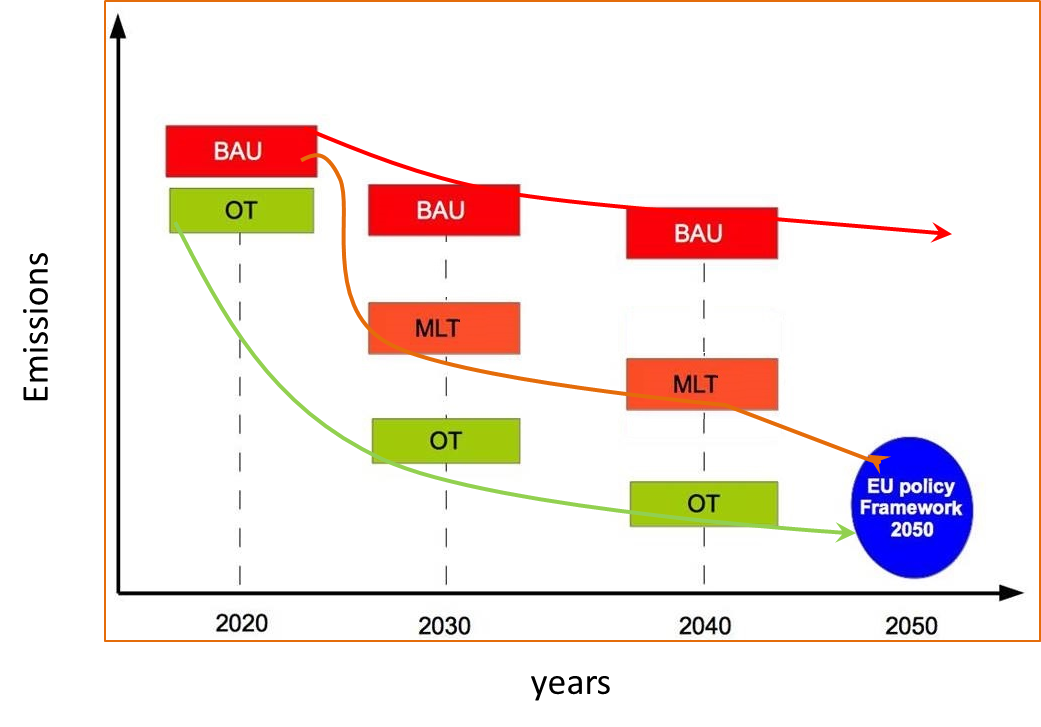
\includegraphics[width=0.8\textwidth]{../resources/images/medeas-scenarios.png}
            \caption{Main scenarios simulated in the MEDEAS IAM}
        \end{figure}
    \end{frame}

    \begin{frame}{Surrogate models}
        Integrating an approximation of a model into the other.
        \begin{figure}
            \centering
            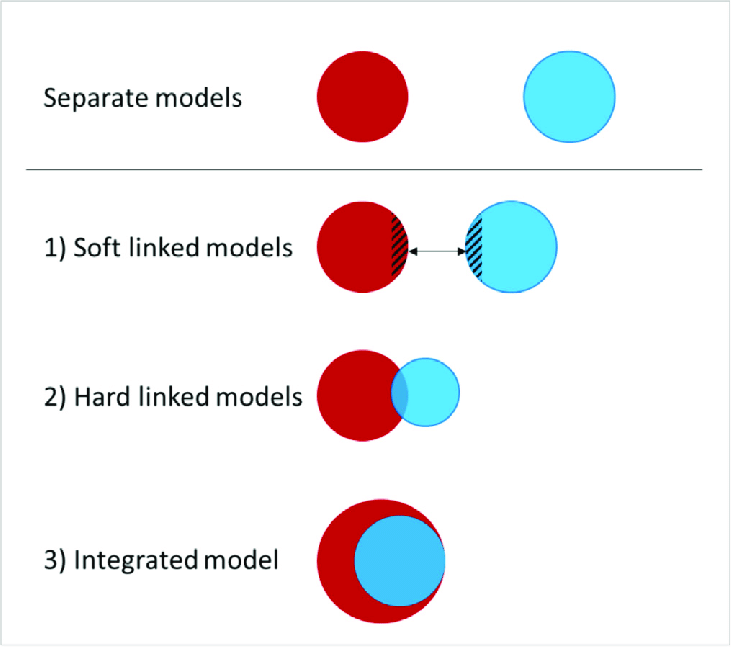
\includegraphics[width=0.5\textwidth]{../resources/images/hybrid_model_variants.png}
            \caption{Illustration of the different linking methods}
        \end{figure}        
    \end{frame}

    \mysection{Dispa-SET simulation and database generation}

    \begin{frame}{Reference simulation and sampling}
        Reference data (mainly demand, availability factors, importations) is from year 2019.

        This simulation is adjusted to fit the desired parameters.

        Latin-Hypercube Sampling is used to maximize the minimum distance between samples.

        The number of points is set to 2400.
    \end{frame}

    \begin{frame}{Variables}
        \begin{table}[h]
            \centering
            \begin{tabular}{|l l l l|}
                \hline
                Variable         & Value  & Lower bound & Upper bound \\ \hline
                CapacityRatio    & 1.658  & 0.5         & 1.8         \\
                ShareFlexibility & 0.418  & 0.01        & 0.99        \\
                ShareStorage     & 0.497  & 0           & 0.5         \\
                ShareWind        & 0.106  & 0           & 0.5         \\
                SharePV          & 0.035  & 0           & 0.5         \\
                rNTC             & 0.282  & 0           & 0.7         \\ \hline
            \end{tabular}
            \caption{Values and bounds of the different variables for the reference simulation in 2019.}
            \label{table:reference-values}
        \end{table}
        The output variables are Curtailment and LoadShedding.
    \end{frame}

    \begin{frame}{Runs and unsuccessful simulations}
        Simulations are run on the NIC5 cluster\footnote{Computational resources have been provided by the Consortium des Équipements de Calcul Intensif (CÉCI), funded by the Fonds de la Recherche Scientifique de Belgique (F.R.S.-FNRS) under Grant No. 2.5020.11 and by the Walloon Region.}.
        
        Simulations featuring $ShareFlexibility$ higher than 0.9014 (around 10\%) stalled, and were discarded. 
    \end{frame}

    \mysection{The surrogate model}

    \begin{frame}{Evaluation of machine learning methods}
        \begin{table}
            \centering
            \begin{tabular}{|l l|}
                \hline
                Method & Best result \\ \hline
                KNN    & 0.04618 \\
                Decision trees & 0.02232 \\
                XGBoost & 0.0053 \\
                Neural networks & 0.0048 \\ \hline
            \end{tabular}
            \caption{Performance of considered machine learning methods}
        \end{table}
        Neural networks are selected.

        Underfitting is preferable to overfitting.
    \end{frame}

    \begin{frame}{Results}
        \begin{figure}[h]
            \centering
            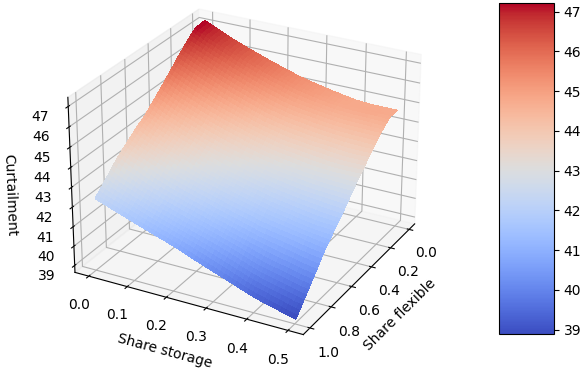
\includegraphics[width=0.8\textwidth]{../resources/images/view_1-2-0.png}
            \caption{Curtailment against share flexibility and share storage}
        \end{figure}
    \end{frame}

    \begin{frame}{Results}
        \begin{figure}[h]
            \centering
            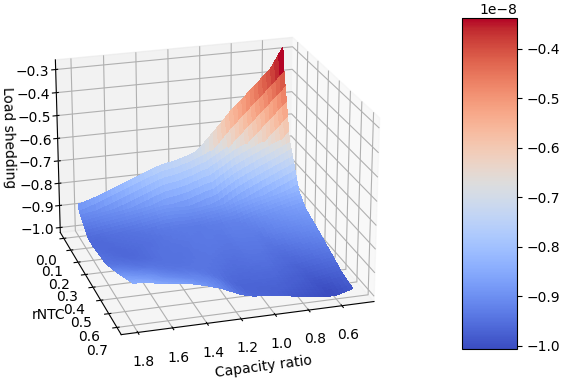
\includegraphics[width=0.8\textwidth]{../resources/images/view_0-5-1.png}
            \caption{Load shedding against capacity ratio and rNTC}
        \end{figure}
    \end{frame}

    \mysection{Integration}

    \begin{frame}{Integration into MEDEAS}
        Integration into Vensim
        \begin{itemize}
            \item With an external function wrapped into a DLL
            \item Easier compatibility and modification of the model
        \end{itemize}
        Use of the python version of MEDEAS with \texttt{pysd}
        \begin{itemize}
            \item Direct use of Tensorflow tools
            \item Harder compatibility
        \end{itemize}
    \end{frame}

    \begin{frame}{Variable linking}
        Links established between the variable in the MEDEAS model and the ones in the surrogate model. $Gen$ stands for generation.
        \begin{table}[h]
            \centering
            \begin{tabular}{|m{2.2cm}|c|}
            \hline 
            Input variable  & Linking equation \\ \hline
            {\color{blue} $share_{PV}$} & {\color{blue} $share_{PV}$ = \color{red} $\dfrac{Gen_{PV}}{Demand_{tot}}$ } \\ \hline 
            {\color{blue} $share_{wind}$} & {\color{blue} $share_{wind}$ = \color{red} $\dfrac{Gen_{wind-onshore} + Gen_{wind-offshore}}{Demand_{tot}}$} \\ \hline 
            {\color{blue} $share_{flexibility}$} & {\color{blue} $share_{flexibility}$} = $40\%$ \\ \hline 
            {\color{blue} $share_{storage}$} & {\color{blue} $share_{storage}$ = \color{red} $\dfrac{Storage_{tot}}{Demand_{tot}}$} $\times 365\times 24$ \\ \hline 
            {\color{blue} $Capacity_{ratio}$} & {\color{blue} $Capacity_{ratio}$ = \color{red} $\dfrac{Gen_{tot}}{Demand_{tot}}$} \\ \hline 
            {\color{blue} $rNTC$} & {\color{blue} $rNTC$ = \color{red} $Growth_{capacity}$} \\ \hline 
            \end{tabular}
            \caption{Variable linking equations. The left-hand side are Dispa-SET variables, and right-hand side MEDEAS variables.}
            \label{tab:linking-equations}
        \end{table}
    \end{frame}

    \mysection{Results analysis}

    \begin{frame}{Comparison}
        \begin{figure}[h]
            \centering
            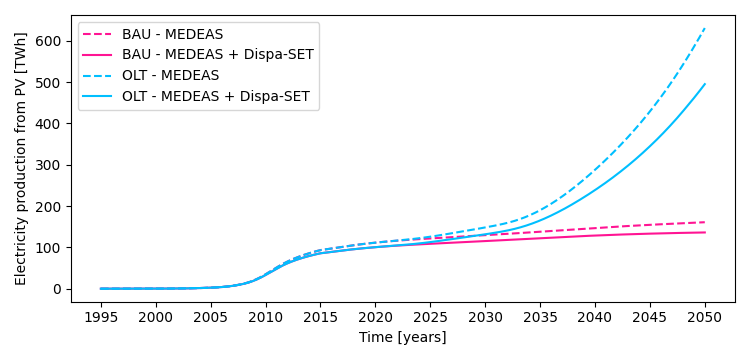
\includegraphics[width=0.8\textwidth]{../resources/images/electricity-production_PV.png}
            \caption{Electricity production predictions from photovoltaic units}
            \label{fig:electricity-production-PV}
        \end{figure}
        Similar results observed for offshore wind production.

        Onshore wind generation also features a maximum that is slightly shifted in time.
    \end{frame}

    \begin{frame}{Comparison}
        \begin{figure}[h]
            \centering
            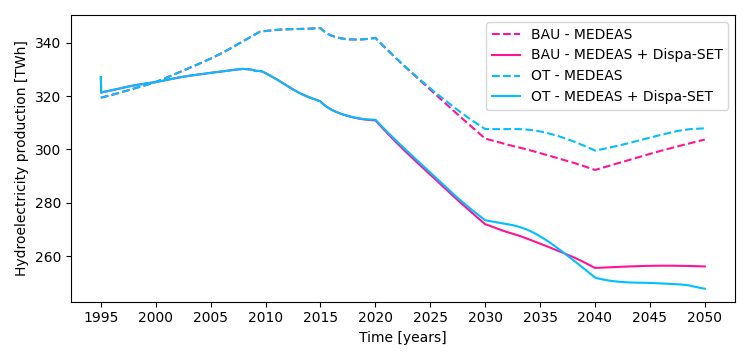
\includegraphics[width=0.8\textwidth]{../resources/images/electricity-production-hydro.png}
            \caption{Electricity production predictions from hydroelectric units}
            \label{fig:electricity-production-hydro}
        \end{figure}
        Hydroelectricity is not favored, due to geographical constraints.
    \end{frame}

    \begin{frame}{Curtailment}
        \begin{figure}[h]
            \centering
            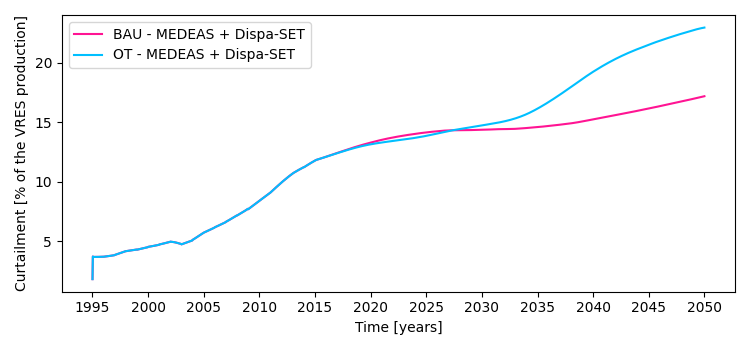
\includegraphics[width=0.8\textwidth]{../resources/images/electricity-production-curtailed.png}
            \caption{Curtailment prediction of the modified MEDEAS for BAU and OLT scenarios}
        \end{figure}

        Curtailment implies indirect emissions.
    \end{frame}

    \begin{frame}{Discussion}
        The integration of the surrogate model leads to a lower prediction of the VRES production.
        
        Likely due to more restrictive constraints, limiting deployment.
    \end{frame}

    \begin{frame}
        Thanks for your attention!
    \end{frame}

\end{document}